\documentclass[11pt]{article}
\usepackage[a4paper,margin=1in]{geometry}
\usepackage[T1]{fontenc}
\usepackage[utf8]{inputenc}
\usepackage{lmodern}
\usepackage{microtype}
\usepackage{amsmath,amssymb}
\usepackage{graphicx}
\usepackage{booktabs}
\usepackage{xcolor}
\usepackage{hyperref}
\usepackage[numbers,sort&compress]{natbib}
\usepackage{caption}
\hypersetup{colorlinks=true,linkcolor=blue!50!black,citecolor=blue!50!black,urlcolor=blue!50!black}
\captionsetup{font=small,labelfont=bf}
\graphicspath{{figures/}}
\setlength{\parskip}{0.25em}
\newcommand{\ci}[2]{[#1,\,#2]}
\newcommand{\todo}[1]{\textcolor{red}{[TODO: #1]}}

\title{Operator Packages, Proposer Strength, and\\ Construction-Family Plateaus in\\ Office-Scale Verified Search}
\author{Roberto I. Ono Filho\\ Independent researcher\\
\texttt{ono.roberto@gmail.com} \quad ORCID \href{https://orcid.org/0009-0006-8650-629X}{0009-0006-8650-629X}}
\date{Draft v0.2 for review, \today}

\begin{document}
\maketitle

\begin{abstract}
Verified search, in which a language model proposes programs, a hard
evaluator scores them, and selection keeps the best, is how machine
systems have recently moved mathematical records; controlled ablations of
the proposer-side components remain rare. We instrument a minimal
FunSearch-style loop at office scale (a 30B local model on a laptop,
120--600 verified samples per run) with three operator packages: a
\emph{schematic notebook} the model writes and carries instead of
verbatim elites, a \emph{named obstacle} (agenda), and \emph{behavioural
repulsion} from constructions already found. On nine construction
problems from a public repository (six in the discovery battery, three in
a prospectively registered extension), the complete $2^3$ factorial with
two replicates supports the primary contrast: the composition closes more
of the seed-to-record gap ($+0.196$ \ci{+0.059}{+0.343}, $p=0.023$
combined; median per-problem effect $+0.045$). Repulsion raises
functional diversity everywhere ($+0.31$, $p=0.0039$; the operator partly
optimizes this quantity). The factorial rejects anchoring as an
interaction (memory$\times$repulsion $\beta\approx 0$): the gain
decomposes additively, the notebook package carrying the largest share,
and a descriptive pattern consistent with collapse prevention remains:
memory+repulsion is the only arm that
never collapses (0 of 18 runs, against 3 for repulsion alone) and matches
the full composition to within $0.025$. A frontier proposer under the
identical loop reaches in tens of samples what the local model does not
in hundreds, and its gains arrive without the operators; once each
proposer reaches its plateau, the tested grid and verifier-time changes
add nothing. The search stalls after
closing $\approx$92\% of the gap toward the best published construction
on the flagship problem, every proposer inside one construction family.
The registered family-hint test gives that reading its first measured
answer on the flagship: named in words, the reference family is adopted
and loses; handed as code, it is optimized but its grid ceiling lies
below the plateau reached unaided. The loop transports and optimizes
ideas; it did not originate one. We release the harness, every
candidate, and the dated pre-registrations.
\end{abstract}

\section{Introduction}
\label{sec:intro}

FunSearch \citep{romeraparedes2024funsearch} and AlphaEvolve
\citep{novikov2025alphaevolve} demonstrated that a language model inside an
evolutionary loop with a hard evaluator can produce genuinely new
mathematical constructions. The systems that followed improved the
\emph{scaffolding}: sample-efficient archives and novelty rejection
\citep{lange2025shinka}, verbal reflections as search gradients
\citep{ye2024reevo}, stronger databases and routing. Two questions have
stayed unmeasured. First, \emph{which parts of what the proposer is asked
to think} (its memory of the lineage, its statement of the obstacle, its
relation to what was already found) change the search, and by how much?
The prompts of the published systems show elite programs verbatim and vary
everything else. Second, \emph{how much of the outcome is the proposer
itself}, holding the loop fixed? Published systems change model and
scaffold together.

This paper measures both, at a scale any laboratory can afford, with the
discipline our earlier studies \citep{ono2026interrupting} found necessary:
every battery pre-registered before running, dated amendments, exact paired
tests, and negative results reported at the same volume as positive ones.
The operators we test are not arbitrary: they are the three interventions
that survived a two-paper program on open-ended generation: a
\emph{schematic memory} (the model's own compressed recap outperformed
verbatim context on document-level integration), a \emph{standing
question}, and \emph{repulsion} from the already-produced, which in weight
space collapsed without an anchor and in behaviour space is the natural
tail-preserving form.

\paragraph{Contributions.}
(1) A pre-registered program of cognitive operators inside a fixed
verified-search loop, grown from a $5{\times}6{\times}2$ ablation to the
complete $2^3{\times}9{\times}2$ factorial: the composition reaches
$+0.196$ ($p=0.023$ over the two-look sequence), behavioural repulsion buys functional diversity in
every problem and replicate ($p=0.0039$), and no single operator is safe
alone.
(2) A revision, by the completed factorial, of this program's recurring
\emph{anchoring pattern}: the memory$\times$repulsion interaction on mean
gap closed is zero: anchoring is not superadditive gain but
\emph{collapse prevention}. Repulsion without memory still breaks (three
collapses in eighteen runs; four when paired with agenda), while
memory+repulsion never does, echoing unanchored preference optimization
in weight space.
(3) A \emph{scaling inversion}: from a 120-sample tie, the composed arm
climbs to 0.3816 at 600 samples while repulsion alone stalls at 0.3514:
diversity without accumulated direction does not compound.
(4) A controlled \emph{proposer comparison}: local 30B versus a frontier
model under the identical loop and budget, on the same problem,
locating the residual gap in the proposer rather than in the loop, with a
frontier-strength scoping run in which the operators' mean contribution
sits inside run-to-run noise.
(5) An honest calibration of office-scale verified search, reaching
57--99.9\% of the reference values (median 89\%) at 120--600 samples,
and a characterized wall: grid resolution,
verifier time and proposer strength each unmoved within the tested
settings, leaving the construction family as the leading suspect for the
binding constraint.

\section{Related work}
\label{sec:related}

\paragraph{Verified search systems.} FunSearch evolved single functions
with small code models and millions of samples
\citep{romeraparedes2024funsearch}; AlphaEvolve evolves whole files with
frontier ensembles and thousands \citep{novikov2025alphaevolve}, and its
repository of 67 problems with official verifiers
\citep{georgiev2025exploration} is the substrate of our experiments.
ShinkaEvolve reports record-level results with $\sim$150 samples using
novelty-based rejection and bandit model selection \citep{lange2025shinka};
ReEvo uses model-written reflections as ``verbal gradients''
\citep{ye2024reevo}. Our schematic notebook differs from ReEvo's
reflections in being a persistent, compressed lineage memory that
\emph{replaces} verbatim elites rather than commenting on pairs. A recent
wave adds persistent memory to evolutionary code search:
$\varepsilon$-MemEvo transfers compact strategy summaries across tasks
with an adaptive injection gate and reports gate ablations
\citep{liu2026memevo}; EvoMem reuses mutation knowledge across runs
\citep{volkov2026evomem}; MEMOIR shares algorithmic and failure-mode
summaries across search branches \citep{haji2026memoir}. What remains
absent, and what we contribute, is a complete factorial, within one task
suite and under a fixed local proposer, of a schematic-notebook package,
an obstacle line, and an exact behavioural duplicate control. LoongFlow \citep{wan2025loongflow} composes planning, hybrid
memory and MAP-Elites niches into one system and reports large efficiency
gains; it is the closest architecture to our composed arm, and exactly the
kind of system whose components an ablation like ours aims to isolate.

\paragraph{Why diversity needs help.} Without selection pressure, LLM
mutation chains collapse into attractor regions \citep{gurkan2026mutation};
RL-tuned models lose pass@$k$ coverage relative to their base
\citep{yue2025rlvr}; and coverage under repeated sampling grows
log-linearly only when a verifier exists \citep{brown2024monkeys}. Our
behavioural-repulsion operator is novelty search
\citep{lehman2011novelty,mouret2015mapelites} transplanted into the
proposer's prompt, with the construction itself (not an embedding) as the
behaviour descriptor.

\section{The harness, the operators, the problems}
\label{sec:harness}

\paragraph{Loop.} A minimal FunSearch-style loop: $K$ islands, each holding
its best programs; per generation, per island, a prompt is built and $S$
candidates sampled; each candidate runs in a sandbox (time and memory
limits) and is scored by the problem's verifier; islands keep bounded
elites and migrate their best every third generation. The proposer is
\texttt{Qwen3-Coder-30B-A3B-Instruct} (8-bit, MLX, on a MacBook M5 Pro)
prompted through its chat template; Section~\ref{sec:records} swaps in
Claude Opus~5 through an API under the identical loop. Every candidate is
logged: code, score, error, generation, island, and a behaviour signature
(a hash of the rounded construction it outputs).

\paragraph{Operators.} \textbf{A} (baseline): the prompt shows the
statement and the island's top-3 programs with scores, FunSearch-style.
\textbf{B} (schematic notebook): each generation the model writes a
$\le$12-line notebook (what worked, what failed and why, the open
question) from the elites and the recent failures; the prompt then
shows the notebook and only the single best program. \textbf{C} (agenda):
one model-written line naming the structural obstacle of the current best,
appended to the prompt. \textbf{D} (behavioural repulsion): candidates
whose construction duplicates an island member's are rejected, and the
prompt lists already-found constructions as forbidden. \textbf{E}: B+C+D. We refer to these as operator \emph{packages}: each
bundles several changes at once (B replaces three verbatim elites with
one, adds failure summaries and an open question, and spends an extra
call; D combines a prompt-level forbidden list with a post-verification
duplicate filter), so the factorial isolates packages, not single
cognitive mechanisms; a finer within-package decomposition is registered
as future work.

\paragraph{Problems.} Nine construction problems ported from the official
repository notebooks, chosen for cheap exact verification and known
headroom. The original battery: circle packing (26 circles, maximize the
sum of radii), ring loading ($m{=}15$, exact $2^m$ verification),
beat-the-average (a pmf maximizing $P[X_1{+}X_2{+}X_3<2X_4]$), the first
autocorrelation inequality (minimize an upper bound on $C_1$),
isosceles-free subsets of the $64^2$ grid, and sum-difference III. A
pre-registered extension, run before any $n{=}9$ analysis, added three:
the max--min pairwise-distance ratio for 16 points in the plane
(minimize), the Heilbronn triangle problem for 11 points (maximize the
smallest triple area), and splitting $180!$ into 180 factors maximizing
the smallest (exact big-integer verification). Each run's budget is 120 verified
samples (10 generations $\times$ 2 islands $\times$ 6); the primary
metric \emph{frac} is the fraction of the seed-to-record gap closed,
\emph{auc} its mean over the budget (sample efficiency), \emph{div} the
share of distinct behaviours among valid candidates.

\section{The factorial}
\label{sec:factorial}

\begin{table}[t]
\centering\small
\begin{tabular}{@{}lcccccccc@{}}
\toprule
frac (pooled over 2 replicates) & A & B & C & D & BC & BD & CD & E \\
\midrule
circle packing 26 & 0.703 & 0.974 & 0.976 & 0.000 & 0.989 & 0.752 & 0.980 & \textbf{0.992} \\
ring loading 15 & 0.444 & 0.767 & \textbf{0.808} & \textbf{0.808} & 0.731 & \textbf{0.808} & \textbf{0.808} & \textbf{0.808} \\
beat-the-average & 0.181 & 0.384 & 0.519 & 0.608 & 0.661 & \textbf{0.789} & 0.540 & 0.709 \\
autocorrelation $C_1$ & 0.059 & 0.156 & 0.041 & 0.202 & 0.014 & \textbf{0.212} & 0.000 & 0.104 \\
isosceles-free $64^2$ & \textbf{0.560} & \textbf{0.560} & \textbf{0.560} & 0.399 & \textbf{0.560} & \textbf{0.560} & \textbf{0.560} & \textbf{0.560} \\
sum-difference III & \textbf{0.392} & 0.329 & 0.253 & 0.158 & 0.314 & 0.327 & 0.069 & 0.362 \\
max--min distance 16 & 0.169 & 0.992 & 0.372 & \textbf{0.993} & 0.919 & 0.793 & 0.247 & 0.708 \\
Heilbronn triangle 11 & 0.672 & 0.431 & 0.507 & 0.540 & 0.371 & 0.477 & 0.619 & \textbf{0.700} \\
$180!$ into 180 factors & \textbf{0.774} & \textbf{0.774} & \textbf{0.774} & \textbf{0.774} & \textbf{0.774} & \textbf{0.774} & \textbf{0.774} & \textbf{0.774} \\
\midrule
mean frac & 0.439 & 0.596 & 0.534 & 0.498 & 0.592 & 0.610 & 0.511 & \textbf{0.635} \\
mean functional diversity & 0.41 & 0.53 & 0.52 & 0.72 & 0.59 & 0.68 & \textbf{0.80} & 0.70 \\
collapses (frac $<$ 0.05, of 18 runs) & 2 & 1 & 1 & 3 & 2 & \textbf{0} & 4 & 1 \\
\bottomrule
\end{tabular}
\caption{The complete $2^3$ factorial over nine problems, pooled over two
independent replicates (120 verified samples per run). frac = fraction of
the seed-to-record gap closed. E has the best mean and is best or
tied-best in five of nine problems; D alone is bimodal: best on wide
valid manifolds (pmfs, sequences), catastrophic where validity is fragile
(packing geometry, constrained integer sets); BD is the only arm that
never collapses, CD the one that collapses most; two problems
(isosceles-free, $180!$) are family plateaus where every arm meets the
same wall.}
\label{tab:factorial}
\end{table}

\begin{figure}[t]
\centering
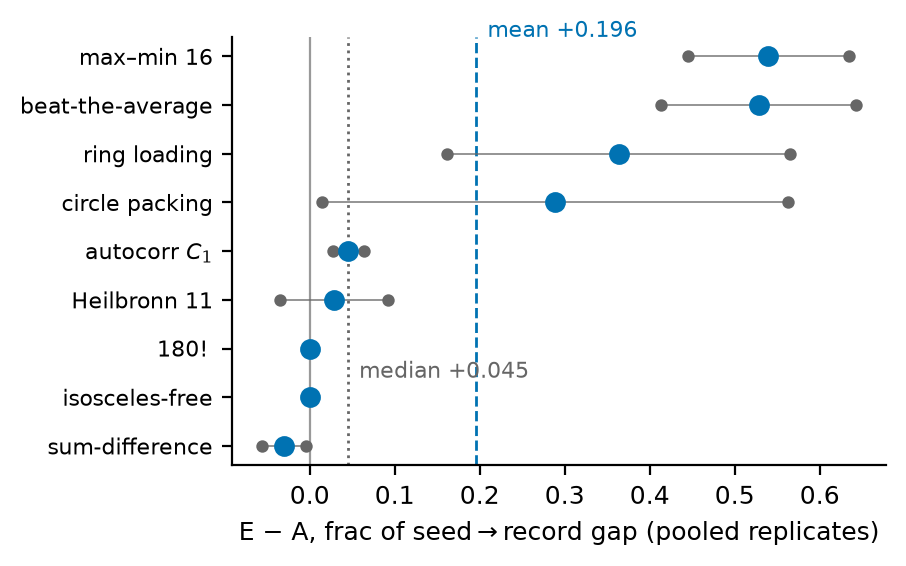
\includegraphics[width=0.6\linewidth]{fig_forest_ea.png}
\caption{The primary contrast, problem by problem: E $-$ A on the
fraction of the seed-to-record gap closed (pooled over two replicates).
Small grey dots are the two replicates (lines join them); the large dot
is their mean. The pooled mean is $+0.196$; the median, $+0.045$;
leave-one-problem-out means stay between $+0.153$ and $+0.224$.
Within-problem replicate spread is large on several problems (circle
packing: $+0.01$ and $+0.56$), which the problem-level test does not
see.}
\label{fig:forest}
\end{figure}

Pre-registered contrasts (exact paired sign-flip over problems, cells =
problems, pooled replicates). The original six-problem battery put the
primary contrast at the design's resolution floor ($+0.199$, $p=0.0625$;
with six cells and one adverse problem the exact test cannot go below
$4/64$); the prospectively registered nine-problem extension supports it:
\textbf{F1} (primary), E vs A on frac: $+0.196$ \ci{+0.059}{+0.343},
$p=0.023$ over the combined nine problems. We report the stages
separately, since the combination is a two-look sequence rather than an
independent confirmation: the three extension problems alone are positive
but underpowered ($+0.19$ on average, $p=0.25$, carried mostly by
max--min distance). The effect is also heterogeneous
(Figure~\ref{fig:forest}): the median per-problem effect is $+0.045$,
leave-one-problem-out means span $+0.153$ to $+0.224$, with large gains
on four problems, little on four, and one small loss.
\textbf{F4}, D vs A on functional diversity: $+0.307$
\ci{+0.149}{+0.477}, $p=0.0039$, the minimum attainable $p$, positive
in all nine problems in both replicates. \textbf{F6} (the anchor), E vs
D: $+0.137$ \ci{-0.047}{+0.382}, $p=0.156$: not supported as a
pairwise contrast; the factorial below resolves what it was measuring.
F2 (auc): $+0.115$, $p=0.070$: the composed arm's advantage builds late.
(The operators' measured overhead is small: one extra call per
island-generation per operator, $\sim$220 characters each, 1--3\% of
proposer output; Section~\ref{sec:limitations} gives the accounting.)

\begin{figure}[t]
\centering
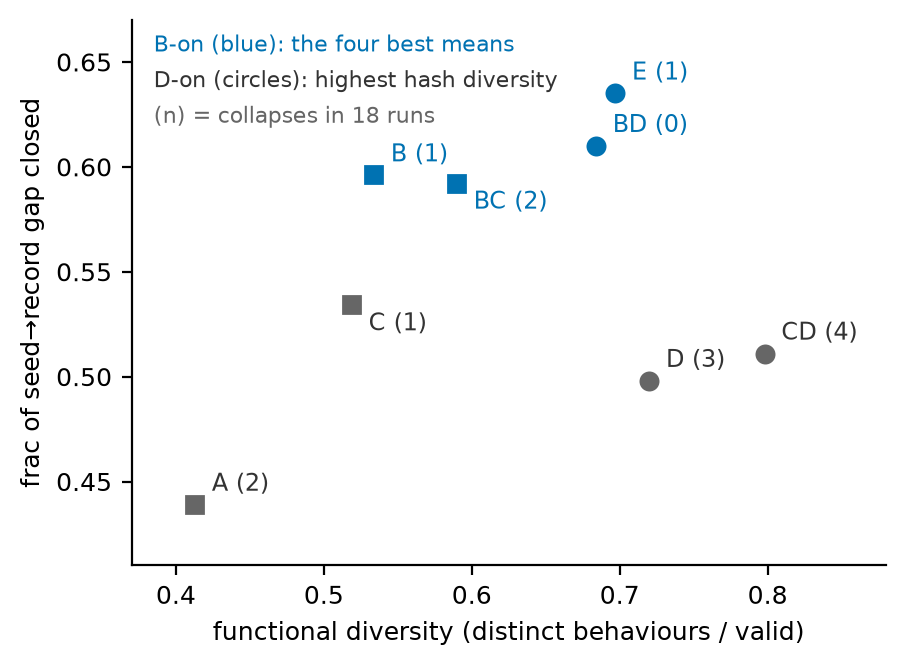
\includegraphics[width=0.62\linewidth]{fig_f23_cube.png}
\caption{The completed $2^3$ at a glance (cell means over nine problems,
two replicates). Memory-on cells (blue) hold the four best gap fractions;
repulsion-on cells (circles) hold the highest functional diversity; the
two axes barely interact ($\beta_{M\times R} \approx 0$). Collapse counts
in parentheses: memory+repulsion is the only arm that never collapses;
agenda+repulsion collapses most.}
\label{fig:cube}
\end{figure}

\paragraph{The completed $2^3$.}
\begin{sloppypar}
Three pairwise arms (memory+agenda, memory+repulsion, agenda+repulsion)
over the same nine problems and two replicates complete the cube
($8$ cells $\times\,9\times2$; pre-registered before running). The
effect-coded analysis (exact sign-flip over problems, $2^9$) rejects the
primary interaction: memory$\times$repulsion $\beta = +0.003$
\ci{-0.039}{+0.035}, $p=0.47$ one-sided; agenda$\times$repulsion is null
($-0.007$, $p=0.79$); and no main effect survives BH correction:
schematic memory is the largest single term ($\beta=+0.057$
\ci{+0.014}{+0.105}, raw $p=0.047$, $q=0.14$), agenda ($+0.016$) and
repulsion ($+0.011$) near zero on frac. The decomposition is exact
($E-A = 2\,(\beta_M+\beta_A+\beta_R+\beta_{MAR}) = 0.196$): the
certified composite gain splits as roughly $58\%$ memory, $16\%$
agenda, $12\%$ repulsion and $14\%$ three-way (a descriptive
decomposition with wide per-term intervals); at $n=9$ the total
certifies, the parts do not. Two patterns in the cube are worth the trip. First, each
operator has one job (Table~\ref{tab:factorial}, Figure~\ref{fig:cube}): the four memory-on
cells hold the four best mean fracs, while every repulsion-on cell sits
at $0.68$--$0.80$ functional diversity against $0.41$--$0.59$ without
it; directionally, memory moves the gap and repulsion moves diversity,
with the caveat that the memory main effect does not survive correction.
Second, the anchor lives in the tail, not the
mean: memory+repulsion is the only arm that never collapses (0 of 18
runs, against 3 for repulsion alone and 4 for agenda+repulsion, the
cube's worst), so what memory buys repulsion is insurance against
starving the island, not superadditive mean gain. Agenda, decomposed at
last, pays for neither: near-zero on frac alone, and the worst collapse
count when paired with repulsion. Exploratory pairwise contrasts back the
parsimony reading: E vs BD $+0.025$ ($p=0.55$, median $0.000$), E vs B
$+0.039$ ($p=0.47$), BD vs B $+0.014$ ($p=0.81$), all null at $n=9$. The
collapse asymmetry is robust to the threshold: at frac $\le 0$, $<0.01$,
$<0.05$ and $<0.10$ the counts stay 3/3/3/3 for repulsion alone and
3/4/4/4 for agenda+repulsion against 0/0/0/0 for memory+repulsion, and
no run anywhere produced zero valid candidates, so these are performance
collapses, not validity collapses.
\end{sloppypar}

The heterogeneity is the finding the factorial adds to the literature:
\emph{where} the valid manifold is wide (a pmf, a sequence of pairs),
repulsion alone is the best single operator; where validity is fragile
(non-overlapping circles, exact integer constraints), it starves the
island (both replicates of circle packing collapse), and the composed
arm inherits most of the benefit with none of the catastrophes. No
single package avoids every failure mode; memory+repulsion was the only
configuration that avoided all of them in these runs.

\section{Scale, proposers, and the wall}
\label{sec:records}

\begin{figure}[t]
\centering
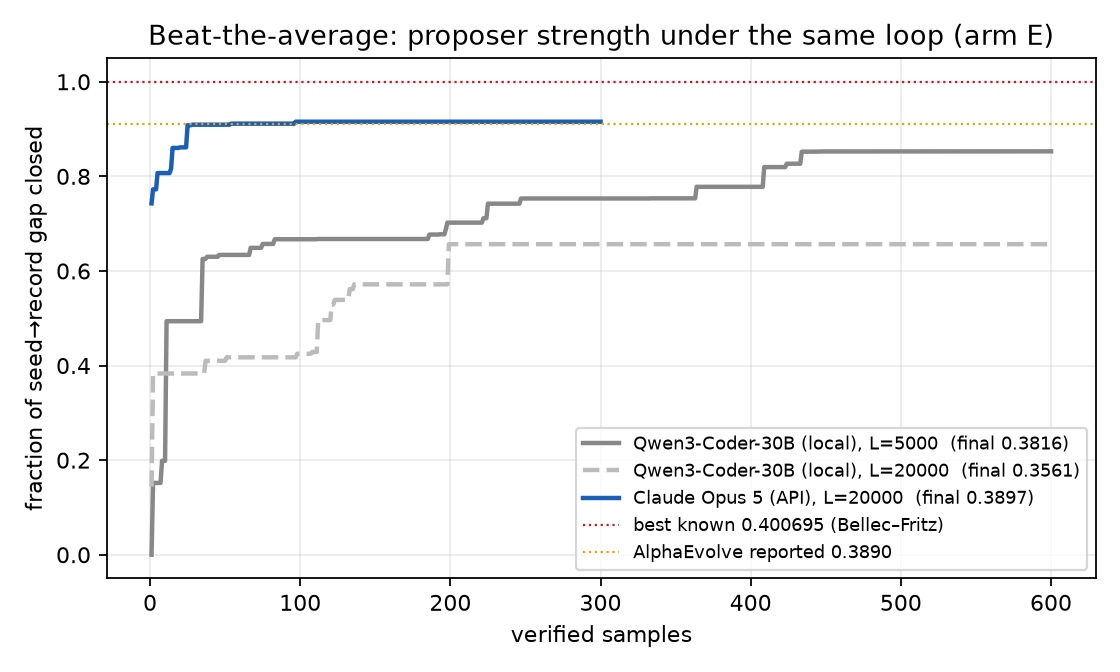
\includegraphics[width=0.86\linewidth]{fig_f4_proposer_curve.png}
\caption{Beat-the-average under the same loop (arm E): fraction of the
seed-to-record gap closed per verified sample. The local 30B at two grid
resolutions; Claude Opus~5; dotted lines mark AlphaEvolve's reported value
(0.3890) and the best known (0.400695, Bellec--Fritz).}
\label{fig:curve}
\end{figure}

We then took the problem with guaranteed headroom, beat-the-average,
where AlphaEvolve's own reported value (0.3890) sits below the best known
(0.400695), and ran a pre-registered ladder. (i) \emph{Budget}: at 600
samples the composed arm reaches 0.3816 while repulsion alone, which had
tied it at 120 samples, stalls at 0.3514: diversity without accumulated
direction does not compound. (The same $5\times$ extension on max--min
distance 16 left both local arms \emph{worse} than their own 120-sample
runs on a fresh seed: seed variance dominates budget there too.)
(ii) \emph{Grid}: refining the pmf grid from
$L{=}5000$ to $L{=}20000$ at equal budget makes the local proposer
\emph{worse} (0.3561): the limit was not resolution. (iii)
\emph{Proposer}: Claude Opus~5 under the identical loop reaches 0.3897
within $\sim$100 samples (just above the repository's published value,
obtained with 2025-era proposers; we read this as locating the
wall, not as ranking systems across model generations) and plateaus
there for 17 generations. (iv) \emph{Verifier time}: tripling the
sandbox budget to 60 seconds, so heavier optimizers can run, moves the
plateau by $+0.0002$.

The constructions are legible. The local model's best is a bimodal sparse
measure of 16 atoms (half the mass on $\{0,1,2,3\}$, geometrically
spaced atoms at the top), with the strategy stated in comments. Claude's
best implements an exact sparse-atom objective with an analytic gradient
and a multiplicative-weights refinement. The frontier proposer and AlphaEvolve's published value sit within
0.0007 of each other; the local model stalls about 0.008 behind them.
All three lie at 92--98\% of the seed-to-reference gap toward a
reference whose construction evidently lies outside the
sparse-atom family every language model proposes. More precisely: the
candidates of both proposers are small finitely supported measures found
numerically, while the \citet{bellec2024beat} construction is a
multiscale, recursively structured sequence of discrete measures whose
analysis shows a finitely supported measure cannot be optimal; the
family-hint conditions below name that structure. Within the settings
tested, grid, time and proposer strength are ruled out; what remains is
the family: an idea.

A second problem sharpens where such ideas live. On max--min distance 16,
the frontier proposer under the same loop emits \emph{in generation
zero}, before any search feedback, a minimax program (SLSQP on
$\min t$ s.t.\ $d^2_{ij}\le t$, $d^2_{ij}\ge 1$, analytic Jacobians)
whose value lies marginally below the repository's published one; every
valid sample across the run converges to the same value. The loop
verified this construction; it did not discover it. We treat the datum as
scope, not as a record claim: the operators structure search and protect
its tails, but they do not inject construction knowledge the proposer
lacks. The pre-registered scoping runs make the same point from the
other side, on all three registered problems. On beat-the-average, the
bare, memory-only and repulsion-only arms land within $0.001$ of one
another ($0.3871$, $0.3866$, $0.3876$; single runs, estimation only) and
within $0.003$ of the composed arm's $0.3897$. On max--min distance and
on the Heilbronn problem every arm converges to an identical value
($12.889230$ and $0.036530$ respectively; the Heilbronn reference in our
registry floors the reported figure, so that value reaches the frozen
reference and supports no exceedance claim). At frontier strength the
operators' mean contribution sits inside run-to-run noise everywhere we
measured it: the certified gains are a local-proposer phenomenon, and
whether the collapse insurance survives at this strength remains
untested.

\section{Discussion}
\label{sec:discussion}

\paragraph{What office scale buys.} With 120--600 verified samples, a
local model and one laptop: 57--99.9\% of the best known values (median
89\%) across nine problems, legible programs, and, with a frontier proposer
at $\sim$US\$50 of API, parity with the values the large systems report on
this problem. The published record-movers used frontier ensembles with
thousands of samples \citep{novikov2025alphaevolve}, millions with small
models \citep{romeraparedes2024funsearch}, or open-source loops with
strong API models \citep{lange2025shinka}; the band we measure (local
proposer, hundreds of samples, controlled operators) was unoccupied,
and it is the band most laboratories can afford.

\paragraph{The operator ledger.} E had the highest mean and one
collapse; memory+repulsion was the only zero-collapse arm, at a mean
within $0.025$ of E's and without the agenda's extra call, so the
parsimonious operational recipe these data support is memory+repulsion,
with the full composition as the highest-mean variant. The mechanism is
visible in the notebooks: the schematic memory keeps direction across
generations and the repulsion spends the saved budget on genuinely
different constructions. Alone, each fails somewhere: memory and agenda
are inert on problems the model already saturates; repulsion starves
fragile manifolds. This is a recurring collapse-prevention pattern,
consistent with the anchoring hypothesis, that this program has now
observed across narrative generation, weight-space preference
optimization, and prompt-space search.

\paragraph{The proposer comparison and the plateau.} On this one problem,
the frontier proposer is far more efficient in verifier evaluations
($+0.008$ absolute over the local model's 600-sample best, reached with
roughly $20\times$ fewer verified samples), and
everything we tried after it moved little (grid, time, more samples:
$+0.0002$). This is a sample-efficiency comparison on one problem under
one harness, not yet a proposer-strength curve; replications on further
problems are planned, and reasoning effort, ensembles, alternative
representations and thousand-sample budgets all remain untested
explanations. The shared plateau suggests, consistently with our
consolidation results \citep{ono2026mass}, that search over a fixed prior
rapidly collects what the prior's construction families contain and then
stalls at the best family member, a hypothesis to test rather than
assert. \emph{The family-hint experiment} (registered before running;
five conditions $\times$ three seeds, 120 samples, memory+repulsion arm)
put it to the test on beat-the-average: (a) no hint; (b) a generic hint;
(c) a structural hint naming the \citet{bellec2024beat} family without
parameters; (d) a crude in-family seed program (score 0.2734); (e) our
best hand instantiation of the family as an oracle seed (0.3742; on this
grid with strict inequality, notably \emph{below} the 0.3816 sparse-atom
plateau, a fact measured and registered before launch). The answer came
with a twist. Condition means over three seeds: no hint 0.352, generic
0.333, structural 0.327 (the worst), family seed 0.358, oracle 0.375.
The structural hint \emph{worked as an instruction and lost as a
search}: its final constructions carry the family's signature (an atom
at zero, atoms accumulating toward the maximum across four
log-distance bands), so the model obeyed, entered a family that is
inferior at this grid, and paid about $0.025$ for it. Handed the family
as code, the loop optimizes it well ($+0.085$ from the crude seed,
above the no-hint endpoint in three of three seeds) and stays loyal to
it (no oracle run deserted to the better sparse family). No unaided run
proposed the family. Within this problem and grid, then, the registered
hypothesis was \emph{not} supported: handing the idea, in words or in
code, did not cross the last mile, and the idea itself was not the
missing step at $L{=}5000$. What the experiment does establish is a
division of labour: the loop transports and optimizes ideas; it does not
originate them, and instructing one is not inducing one, the third
appearance of that pattern in this program (the continuity connective of
the companion study; the frontier scoping runs; now the structural
hint). This is the question \citet{georgiev2025exploration} report
answering with an expert in the loop, from the other side.

\paragraph{Design rules.} For verified search at small scale: pair
memory with repulsion (the zero-collapse arm; the full composition adds
$+0.025$ of mean at the cost of the agenda's extra calls, a difference
our data cannot distinguish from zero), and never run repulsion alone on
fragile manifolds; keep the
behaviour descriptor exact (the construction, not an embedding); spend on
the proposer before spending on samples; treat plateaus as candidate family
boundaries and test them (grid, time, proposer and hints in
pre-registered steps) rather than declaring them.

\section{Experimental provenance}
\label{sec:provenance}

Every battery was registered before running; the combined analyses are
sequential, and the table makes the order of looks explicit.

\begin{table}[h]
\centering\small
\begin{tabular}{@{}lllll@{}}
\toprule
battery & registered & data already seen & primary & status \\
\midrule
F ($5{\times}6{\times}2$) & 2026-08-22 & none & E$>$A frac & $p=0.0625$ (floor) \\
F-ext ladder & 2026-08-23 & F & budget/grid/proposer & descriptive \\
F-ext2 ($n{=}9$) & 2026-08-24 & F, ladder & E$>$A frac & $p=0.023$ combined \\
$2^3$ completion & 2026-08-24 & F, ext2 partial & M$\times$R $>0$ & rejected ($p=0.47$) \\
Frontier scoping & 2026-08-26 & all above & estimation only & operators $\approx$ null \\
Family hint & 2026-08-27 & all above & optimize-once-given & yes as code, no as words \\
\bottomrule
\end{tabular}
\caption{Order of registrations and looks. The nine-problem primary
analysis is a two-look sequence (discovery + prospective extension), not
an independent confirmation.}
\label{tab:provenance}
\end{table}

\section{Limitations}
\label{sec:limitations}

Nine problems is still a small universe of construction families; the
full $2^3$ isolates interactions, but at $n{=}9$ no per-term effect
survives correction, so the operator decomposition (memory largest) is
directional, not certified, and the collapse asymmetry is descriptive;
budgets are equalized in proposals and verifier evaluations (120 of each
per run; duplicate rejection in the repulsion arms happens after
verification, since the signature requires the construction, and discards
20--30 verified candidates per run from the islands); the operators'
extra calls are measured at one per island-generation per operator
($\sim$220 characters per call, an overhead of 1--3\% of proposer
output characters), so sample efficiency here means verifier-evaluation
efficiency at nearly matched token budgets; the diversity
metric is related to the repulsion operator's own filter; the behaviour
signature is a hash of the returned construction after rounding, with no
canonicalization for symmetries (permutation, rotation, reflection), so
div can count symmetric variants as distinct, its rounding sensitivity is
untested, and the D filter and the div metric share this signature; the six
problems satisfy criteria fixed before any runs (cheap exact verifier,
short-function candidates, known headroom; the universe of 68 candidate
problems
and per-problem ratings are in the released reconnaissance table) but were
not sampled randomly; \emph{frac} is floored at the seed by construction,
signs are harmonized for minimization, and reference values are frozen at
the repository commit recorded in the release; the scaling ladder is one
domain; the API proposer is not bitwise reproducible and its reasoning
effort was fixed low; comparisons against repository values compare a
2026 proposer with values obtained by 2025-era systems, so they locate
our wall and never rank systems: no system-level head-to-head with
ShinkaEvolve or AlphaEvolve is attempted, and the operators should be
read as structuring search, not as a substitute for construction
knowledge the proposer lacks.

\section{Conclusion}
\label{sec:conclusion}

Inside a fixed verified-search loop at office scale, the operator
packages our generation studies isolated (a schematic notebook, a named
obstacle, behavioural duplicate control) compose into the arm with the
highest mean, E, at one collapse in eighteen runs; memory+repulsion was
the only zero-collapse configuration, within $0.025$ of E's mean, and is
the parsimonious recipe these data support. Repulsion alone enforces
behavioural non-duplication by construction and was the best single
package exactly where the valid manifold is wide; and on the one problem
where we compared them, a frontier proposer reached a higher value with
roughly $20\times$ fewer verifier evaluations. On beat-the-average both
proposers stalled inside one small finite-support construction family,
below a multiscale reference; the other plateaus are consistent with,
but do not establish, analogous family boundaries. Whether
crossing that boundary requires what we have informally called an idea
was put to a registered test on the flagship problem: the idea, handed in
words, was followed and lost; handed as code, it was optimized but its
grid ceiling lies below the plateau the models reach unaided. The loop
moved ideas; it did not originate one, and the one we handed it was not
the missing mile here. Whether the last mile of these searches is an
idea, the question this program has carried informally, remains open,
now with its first measured answer.

\bibliographystyle{plainnat}
\bibliography{references}

\end{document}
